\section{Introduction and Planning}
\subsection{Tiberius II}
\label{sec:Mech_IP_Tib2}

This group's involvement in the Tiberius project began with Tiberius II - a four-wheeled fixed-axis variant of the robot. Comprised of an aluminium extrusion frame, four wheels and motors, a large battery pack and a number of sensors and other smaller components, this was a simplistic design from a mechanical standpoint.
\begin{figure}[!htb]
\begin{center}
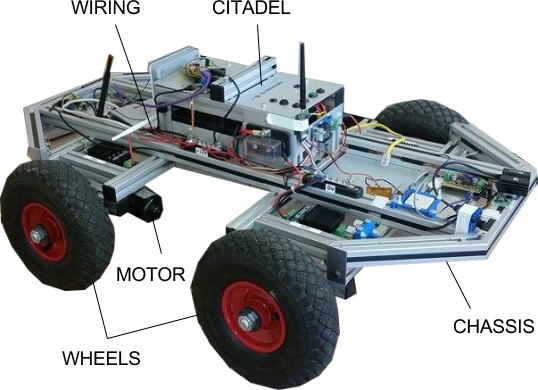
\includegraphics[width=10cm]{mech_Tib_old_diagram.png}
\end{center}
\caption{Tiberius II}
\label{fig:mech_old}
\end{figure}
\newline
However, the group unanimously decided that there was room for improvement. The aluminium frame, while simple at first glance, was in fact over-designed; using far more material than required, making the robot unnecessarily heavy and components difficult to remove or replace.
\newline
In a similar fashion the wheel and motor system left much to be desired. While simple to use, the `tank style' steering caused excessive vibrations as the robot skidded around, and the direct drive link between the motor and the wheel meant that the coupling between the motor and the wheel shaft took the full weight of the robot. Over time this caused the threads on the wheel shaft to be destroyed, eventually leading the the complete disconnection of the motor from the wheel. The bulky motors mounted low-down and in line with the wheels also lowered Tiberius' ground clearance (\textit{see figure \ref{fig:mech_gnd}}). They were likely to catch on obstacles or rough terrain, causing abrasive damage.
\begin{figure}[!htb]
\begin{center}
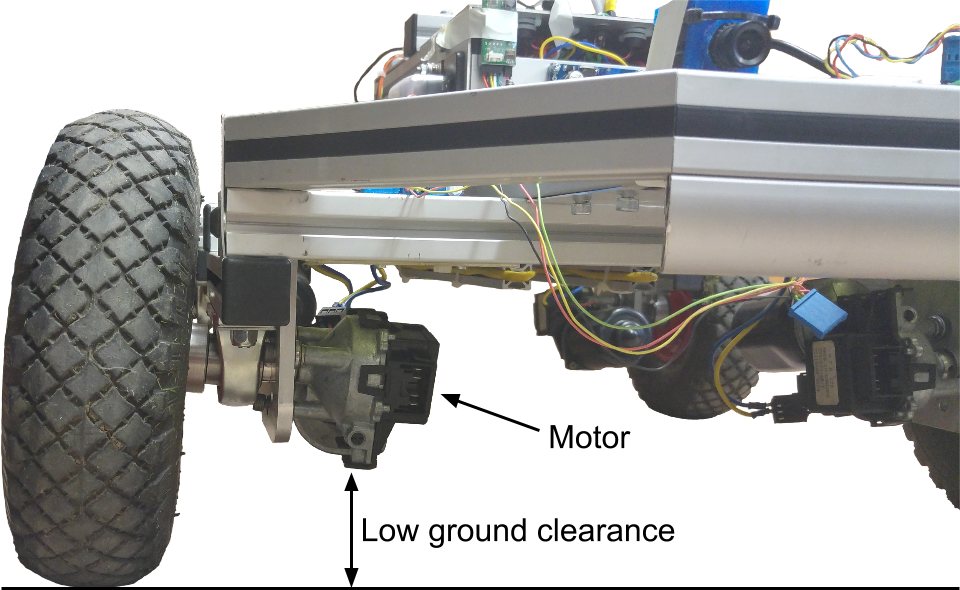
\includegraphics[width=10cm]{mech_ground_clearance.png}
\end{center}
\caption{Underside of Tiberius II}
\label{fig:mech_gnd}
\end{figure}
\newline
Clearly with so many changes it was likely that the entire structure of the robot would have to be changed. However, this opened up the opportunity to think about further mechanical features that would have been harder to implement while keeping the old robot intact. Drastic changes such as the addition of a steering system or shock absorbers to the frame would now be possible.
\newline
With so many opportunities for change in the pipeline it was decided that this project would culminate in an entirely new version of the Tiberius robot - dubbed `Tiberius III'.
\newpage
\subsection{Aims and Objectives}
With practically endless options for changing the design, it was important to plan our objectives carefully, keeping in mind the time constraints of the project. Three main areas for improvement were identified:

\begin{enumerate}
\item Motors
\begin{itemize}
\item \textbf{New DC motors}
\newline
As stated above, there were some issues with the motors on Tiberius II. As such, new motors were provided at the commencement of the project with the expectation that we would integrate them into the new design. These new DC motors had several inherent advantages over the old ones that will be discussed fully in Section \ref{sec:Mech_BGT_Motor}.

\item \textbf{Velocity control}
\newline
The previous version of Tiberius relied on the idea that identical motors should run at the same speed, and thus the robot will drive in a straight line. From a practical point of view this is of course untrue as no piece of equipment is perfect, and the robot had a tendency to veer off-track. To amend this issue, some sort of velocity control system would need to be implemented, using feedback to ensure that the motors matched each other in speed. This could also be used to further control the rate of turn.
        
\item \textbf{mbed control units}
\newline
The last item regarding the motors themselves was linked to the previous; the velocity control would have to be controlled by individual mbeds on each motor.
\end{itemize}

\item Wheel mounting
\begin{itemize}
\item \textbf{Wheel unit}
\newline
Modularity of components was a problem that was identified early on - Tiberius II was difficult to adapt or modify. With regards to the wheels, it would be beneficial to design an all-in-one unit encompassing the wheels, motors, and the components dealing with velocity control as mentioned above. This unit could be replicated for all four wheels and easy to replace.
\item \textbf{Steering}
\newline
In order to improve Tiberius' capabilities, it was decided that some sort of steering system should be implemented - either on the two front wheels, or alternatively on all four. This would allow much smoother turning, and opens the possibility of Bezier curve-based path planning.\cite{Dun_bezier}
\item \textbf{Suspension}
\newline
Tiberius II had some problems traversing rough ground; while it had more than enough torque to traverse relatively large objects like pavement kerbs, it could not do this smoothly and could bounce wildly while travelling. This in turn had the potential to damage some components. In order to reduce wear and tear it was decided that shock absorbers should be added to all four wheel units. This would have the added bonus of increasing Tiberius' ride height and hopefully allowing it to traverse even larger obstacles.
\end{itemize}

\item Chassis
\begin{itemize}
\item \textbf{Reduced chassis}
\newline
As stated above, Tiberius II used an excessive amount of material in its chassis. With the possibility of an entirely new frame, it would be possible to reduce the amount of negligible material used. At the same time, 3D printing technology would be used to create plastic mounts for all components, further reducing the need for heavy metal attachment points.
\item \textbf{Improved wiring standards}
\newline
Considering some of the other objectives in place with regards to power management and new components, it was highly likely that a lot more wiring would be required. This necessitated the application of some wiring standards; cable management to keep everything tidy and make it easier to diagnose problems, and colour-coded wiring representing different voltages or data.
\item \textbf{Finalised design iteration}
\newline
As a concatenation of the above objectives, the primary goal was to make this the final mechanical iteration of the Tiberius robot, which all future groups would expand upon.
\end{itemize}
\end{enumerate}